% Diese Datei ist Teil des Buchs "Schreibe Dein Programm!"
% Das Buch ist lizensiert unter der Creative-Commons-Lizenz
% "Namensnennung - Weitergabe unter gleichen Bedingungen 4.0 International (CC BY-SA 4.0)"
% https://creativecommons.org/licenses/by-sa/4.0/deed.de

\chapter{Daten mit Selbstbezug}
\label{cha:selbstbezug}

Zusammengesetzte und gemischte Daten sind die Hauptorganisationsformen
für Daten.  Allerdings haben wir bisher nur Daten vorgestellt, die
feste Größe haben und damit im Wortsinn beschränkt sind.  Viele
Informationen haben aber variable Größe: Die Bücher im Regal werden
immer mehr, Bauwerke bestehen aus variable vielen Bauteilen.  Um
solche Informationen als Daten zu repräsentieren, stellen wir in
diesem Kapitel eine weitere Technik der Datenmodellierung vor, den
\textit{Selbstbezug}\index{Selbstbezug}.  Hier sind einfache Beispiele:
%
\begin{itemize}
\item Ein Fluss besteht aus Hauptfluss und Nebenfluss~-- beides wieder
  Flüsse.
\item Ein Dateiverzeichnis auf dem Computer kann 
  Unterverzeichnisse enthalten.
\item Ein großer Bücherstapel besteht aus einem etwas kleineren
  Bücherstapel und einem weiteren Buch.
\end{itemize}

\section{Flüsse modellieren}

\begin{figure}[tbh]
  \centering
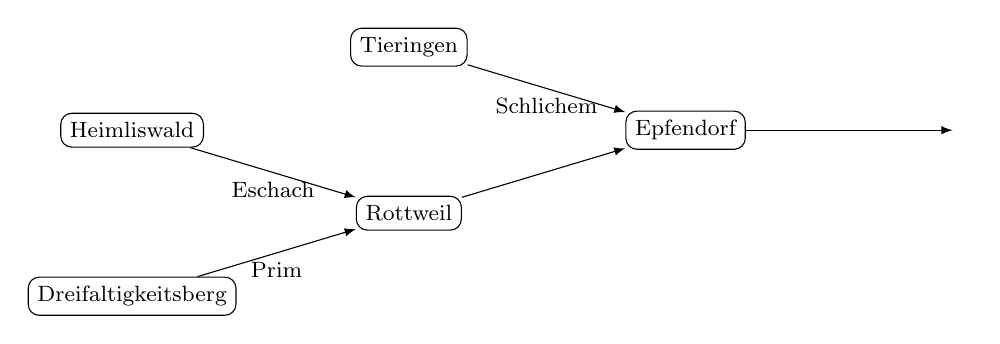
\begin{tikzpicture}
  [
    confluence/.style = {shape=rectangle, rounded corners,
                         draw, align=center},
    absent/.style = {},
    grow                    = left,
    sibling distance        = 6em,
    level distance          = 10em,
    % makes arrows the opposite direction from -latex
    edge from parent/.style = {draw,latex-},
    every node/.style       = {font=\footnotesize}
    ]
    \node [absent] {}
    child {
      node [confluence] {Epfendorf}
        child {
          node [confluence] {Tieringen}
          edge from parent node [below] {Schlichem} }
        child { node  [confluence] {Rottweil}
          child { node [confluence] {Heimliswald}
            edge from parent node [below] {Eschach} }
          child { node [confluence] {Dreifaltigkeitsberg}
            edge from parent node [below] {Prim} } } };
\end{tikzpicture}
  \caption{Der Neckar nahe der Quellen}
  \label{fig:neckar}
\end{figure}

\noindent Abbildung~\ref{fig:neckar} ist ein Diagramm, das die
Struktur des Neckar nahe der Quellen beschreibt: Er fließt zunächst
aus den Bächen Eschach und Prim zusammen, und danach fließen immer
weitere Bäche und Flüsse hinzu~-- in der Abbildung noch die
Schlichem.

Die Struktur eines Flusses werden wir durch Daten abbilden, um danach
eine Funktion zu schreiben, die feststellt, ob ein Fluss durch einen
bestimmten Ort fließt.  Unser erster Versuch einer Datendefinition
sieht so aus:
%
\begin{lstlisting}
; Ein Fluss kommt entweder aus:
; - einer Quelle
; - einem Hauptfluss und einem Nebenfluss
\end{lstlisting}
%
Man kann zwar schon sehen, dass es sich um eine Fallunterscheidung
handelt, aber wir können die Formulierung schärfen, um klar zu machen,
dass es sich um gemischte Daten handelt:
%
\begin{lstlisting}
; Ein Fluss ist eins der folgenden:
; - ein Bach aus einer Quelle
; - ein Zusammentreffen von einem Hauptfluss und einem Nebenfluss
\end{lstlisting}
%
Daraus können wir direkt eine Signaturdefinition machen:
%
\begin{lstlisting}
(define river
  (signature (mixed creek confluence)))
\end{lstlisting}
%
Die Datendefinitionen für "<Bach"> und "<Zusammentreffen"> fehlen
allerdings noch.  In Abbildung~\ref{fig:neckar} steht an den Bächen
jeweils noch der Name.  Eine passende Datendefinition sieht so aus:
%
\begin{lstlisting}
; Ein Bach hat folgende Eigenschaften:
; - Ursprungsort
\end{lstlisting}
%
Das klingt ein bißchen komisch, weil der Bach ja nur \emph{eine}
Eigenschaft hat, aber die Datendefinition trotzdem zusammengesetzte
Daten beschreibt.  Trotzdem ist das legitim und korrekt~-- niemand
wird sagen wollen, dass der Ursprungsort der Bach \emph{ist}.
Außerdem kannst Du Dir vorstellen, dass ein Bach später noch mehr
Eigenschaften bekommt, die wir in den Daten festhalten
wollen. (Wasserqualität oder Fließgeschwindigkeit zum Beispiel.)
Entsprechend ist es auch sinnvoll, dafür eine Record-Definition zu
schreiben:
%
\begin{lstlisting}
(define-record-functions creek
  make-creek
  creek?
  (creek-origin string))
\end{lstlisting}
%
Wenn später noch weitere Eigenschaften hinzukommen, können wir die
Record-Definition erweitern, ohne anderen Code zu beeinträchtigen.

Kommen wir zu den Zusammentreffen.  Auch hier ist ein Ort relevant~--
dort, wo sie zusammentreffen.  Außerdem ist wichtig, \emph{welche}
Flüsse oder Bäche da zusammentreffen.  Die Datendefinition könnte so
aussehen:
%
\begin{lstlisting}
; Ein Zusammentreffen besteht aus:
; - Ort
; - Hauptfluss
; - Nebenfluss
\end{lstlisting}
%
Die Formulierung zeigt eindeutig, dass es sich um zusammengesetzte
Daten handelt.  Aber diese Datendefinition weist eine Auffälligkeit
auf, die erst sichtbar wird, wenn wir sie im Zusammenhang der
Gesamt-Datendefinition für Flüsse betrachten:
%
\tikzstyle{every picture}+=[remember picture]
\tikzstyle{fluss} = [shape=rectangle,inner sep=0pt,text depth=0pt]
%
\begin{lstlisting}
; Ein |\tikz\node[fluss](fluss){\textbf{Fluss}};| ist eins der folgenden:
; - |\ldots|
; - ein Zusammentreffen |\ldots|
|\ldots|
; Ein Zusammentreffen besteht aus:
; - Ort
; - Haupt|\tikz\node[fluss](fluss1){\textbf{fluss}};|
; - Neben|\tikz\node[fluss](fluss2){\textbf{fluss}};|
\end{lstlisting}
%
\begin{tikzpicture}[overlay]
  \path[->,blue,thick](fluss1) edge [out=0, in=0] (fluss);
  \path[->,blue,thick](fluss2) edge [out=0, in=0] (fluss);
\end{tikzpicture}
%
Die Datendefinition für "<Fluss"> benutzt selbst den Begriff
"<Fluss">.   Noch offensichtlicher wird das, wenn wir die dazu
passende Record-Definition erstellen:
%
\begin{lstlisting}
(define-record-functions confluence
  make-confluence
  confluence?
  (confluence-location  string)
  (confluence-main-stem river)
  (confluence-tributary river))
\end{lstlisting}
%
In der Definition von \texttt{confluence} wird \texttt{river} benutzt
und umgekehrt.  Das ist nichts schlimmes~-- im Gegenteil, diese beiden
\textit{Selbstbezüge}\index{Selbstbezug} erlauben uns, ganz
unterschiedliche Flüsse zu beschreiben, insbesondere solche
unterschiedlicher Größe.  Den Abschnitt des Neckar in~\ref{fig:neckar}
können wir so abbilden:
%
\begin{lstlisting}
(define eschach (make-creek "Heimliswald")) ; Quelle des Neckar
(define prim (make-creek "Dreifaltigkeitsberg")) ; Quelle des Neckar
; erster Zusammenfluss des Neckar:
(define neckar-1 (make-confluence "Rottweil" eschach prim))
; Zufluss des Neckar:
(define schlichem (make-creek "Tieringen")) 
; zweiter Zusammenfluss des Neckar:
(define neckar-2 (make-confluence "Epfendorf" neckar-1 schlichem))
\end{lstlisting}
%
Wir hatten angekündigt, eine Funktion zu schreiben, die feststellt, ob
ein Fluss durch einen bestimmten Ort fließt.  Wir machen das wieder
nach Vorschrift, also zuerst die Kurzbeschreibung:
%
\begin{lstlisting}
; Fließt Fluss durch den angegebenen Ort?
\end{lstlisting}
%
In der Kurzbeschreibung sind schon die Substantive "<Fluss"> und
"<Ort"> als Eingaben aufgeführt, die übertragen wir in die Signatur.
Da die Funktion eine Ja-/Nein-Frage beantwortet, liefert sie einen
booleschen Wert und hat ein Fragezeichen hinten am Namen:
%
\begin{lstlisting}
(: flows-through? (river string -> boolean))
\end{lstlisting}
%
Bei den Tests achten wir darauf, dass wir sowohl Bäche als auch Flüsse
testen, und sowohl Fälle, bei denen \lstinline{#t} als auch solche,
bei denen \lstinline{#f} herauskommt:
%
\begin{lstlisting}
(check-expect (flows-through? eschach "Heimliswald") #t)
(check-expect (flows-through? eschach "Tübingen") #f)
(check-expect (flows-through? neckar-2 "Heimliswald") #t)
(check-expect (flows-through? neckar-2 "Rottweil") #t)
(check-expect (flows-through? neckar-2 "Berlin") #f)
\end{lstlisting}
%
Das Gerüst ergibt sich wie immer direkt aus der Signatur:
%
\begin{lstlisting}
(define flows-through?
  (lambda (river location)
    ...))
\end{lstlisting}
%
Da es sich bei \lstinline{river} um gemischte Daten handelt, können
wir die Schablone dafür ergänzen.  Da \lstinline{river} zwei Fälle hat
(Bäche und Zusammenflüsse), muss die Schablone zwei Zweige haben.  Die
Bedingungen sind Aufrufe der jeweiligen Prädikate für
\lstinline{creek} und \lstinline{confluence}:
%
\begin{lstlisting}
(define flows-through?
  (lambda (river location)
    (cond
      ((creek? river) ...)
      ((confluence? river) ...))))
\end{lstlisting}
%
Nun können wir Code für die beiden Zweige ergänzen.  Fangen wir mit
den Bächen an.  Da es sich bei \lstinline{creek} um zusammengesetzte
Daten handelt (mit nur einem Bestandteil), sollte der Aufruf des
Selektors im Rumpf vorkommen:
%
\begin{lstlisting}
(define flows-through?
  (lambda (river location)
    (cond
      ((creek? river)
       ... (creek-origin river) ...
      ((confluence? river)
       ...))))
\end{lstlisting}
%
Der Selektor \lstinline{creek-origin} hat einen Ursprungsort.  Wenn dieser dem
gesuchten Ort entspricht, so fließt der Fluss durch diesen Ort, sonst
nicht.  Im ersten Fall sollte \lstinline{#t} herauskommen, im zweiten
\lstinline{#f}.  Das sieht so aus:
%
\begin{lstlisting}
(define flows-through?
  (lambda (river location)
    (cond
      ((creek? river)
       (if (string=? (creek-origin river) location)
           #t
           #f))
      ((confluence? river)
       ...))))
\end{lstlisting}
%
Dieser Code kann noch etwas vereinfacht werden: Der
\lstinline{if}-Ausdruck sagt ja salopp formuliert:
%
\begin{quote}
  Wenn \lstinline{(string=? (creek-origin river) location)} als
  Resultat \lstinline{#t} liefert, dann \lstinline{#f}, und wenn es
  \lstinline{#f} liefert, dann \lstinline{#f}.
\end{quote}
%
Da reicht es auch, \lstinline{(string=? (creek-origin river) location)} hinzuschreiben.
%
\begin{aufgabe}\label{aufgabe:iftruefalse}
  Kannst Du diese Vereinfachung auf \lstinline{if}-Ausdrücken
  verallgemeinern und als Gleichung schreiben?
\end{aufgabe}
%
Als nächstes können wir uns um den anderen Fall kümmern,
\lstinline{confluence}.  Auch dort handelt es sich um
zusammengesetzte Daten, wir können also schon einmal die
Selektoraufrufe hinschreiben:
%
\begin{lstlisting}
(define flows-through?
  (lambda (river location)
    (cond
      ((creek? river)
       (string=? (creek-origin river) location))
      ((confluence? river)
      ...
       (confluence-location river)
       (confluence-main-stem river)
       (confluence-tributary river)
       ...))))
\end{lstlisting}
%
Soweit die Schablone, wir können uns also Gedanken zur eigentlichen
Aufgabe machen.

Als erstes steht da \lstinline{(confluence-main-stem river)} der Ort
des Zusammenflusses.  Wenn es sich dabei um den gesuchten Ort handelt,
können wir die Frage, ob der Fluss durch diesen Ort fließt, bereits
mit "<ja"> beziehungsweise \lstinline{#t} beantworten:
%
\begin{lstlisting}
(define flows-through?
  (lambda (river location)
    (cond
      ((creek? river)
       (string=? (creek-origin river) location))
      ((confluence? river)
       (if (string=? (confluence-location river) location)
           #t
           ...
           (confluence-main-stem river)
           (confluence-tributary river)
           ...)))))
\end{lstlisting}
%
Aber was wenn nicht?  Dann müssen wir uns an die beiden anderen
Selektor-Aufrufe halten, die uns den Haupt- und den Nebenfluss des
Zusammenflusses liefern.  Wenn der eine oder der andere durch den
gesuchten Ort fließt, dann könnten wir die Frage unserer Funktion
ebenfalls mit "<ja"> beantworten.  Dazu müssten wir also feststellen:
%
\begin{enumerate}
\item Fließt der Hauptfluss durch den Ort \lstinline{origin}?
\item Fließt der Nebenfluss durch den Ort \lstinline{origin}?
\end{enumerate}
%
Nun, wir schreiben ja gerade eine Funktion, die feststellt, ob ein
Fluss durch einen bestimmten Ort fließt.  Können wir die benutzen?
Wir schreiben das mal hin:
%
\begin{lstlisting}
(define flows-through?
  (lambda (river location)
    (cond
      ((creek? river)
       (string=? (creek-origin river) location))
      ((confluence? river)
       (if (string=? (confluence-location river) location)
           #t
           ...
           (flows-through? (confluence-main-stem river) location)
           (flows-through? (confluence-tributary river) location)
           ...)))))
\end{lstlisting}
%
Die beiden Aufrufe von \lstinline{flows-through?} entsprechen gerade
den beiden Fragen von oben.  Wir können ihre Ergebnisse kombinieren,
um unsere Antwort zu errechnen: Wenn der Hauptfluss durch
\lstinline{location} fließt \emph{oder} der Nebenfluss durch
\lstinline{location} fließt, so fließt auch der "<Gesamtfluss"> durch
\lstinline{location}.  So sieht das aus:
%
\begin{lstlisting}
(define flows-through?
  (lambda (river location)
    (cond
      ((creek? river)
       (string=? (creek-origin river) location))
      ((confluence? river)
       (if (string=? (confluence-location river) location)
           #t
           (or
            (flows-through? (confluence-main-stem river) location)
            (flows-through? (confluence-tributary river) location)))))))
\end{lstlisting}
%
Fertig!

In dieser Funktion passiert etwas besonderes, das es in den
Funktionen davor noch nicht gab: Sie enthält einen Aufruf von sich
selbst, einen sogenannten \textit{rekursiven Aufruf\index{rekursiver
    Aufruf}}.  Diese rekursiven Aufrufe sind genau an den Stellen, wo
die Datendefinition von \lstinline{river} Selbstbezüge enthält.

Das ist kein Zufall: Nahezu alle Funktionen, die Daten mit
Selbstbezügen konsumieren, enthalten an den Stellen der Selbstbezüge
rekursive Aufrufe.  Daraus machen wir eine Schablone:
%
\begin{konstruktionsanleitung}{Selbstbezüge als Eingabe: Schablone}
  \label{ka:selbstbezug-schablone}
  Wenn Du eine Funktion schreibst, die Daten konsumiert, in denen
  Selbstbezüge enthalten sind, dann schreibe an die Stellen der
  Selbstbezüge jeweils einen rekursiven Aufruf.
\end{konstruktionsanleitung}
%
Ein Nachtrag noch: Der \lstinline{if}-Ausdruck in der
\lstinline{flows-through?}-Funktion passt \emph{fast} auf das Muster
aus Aufgabe~\ref{aufgabe:iftruefalse}.  Der einzige Unterschied ist,
dass in der Alternative der Verzweigung nicht \lstinline{#f} steht.
Allgemein wir ein solcher \lstinline{if}-Ausdruck folgendermaßen
ausgewertet:
%
\begin{lstlisting}
(if |$b$| #t |$a$|)
|\evalsto| #t ; falls |$b=$| #t
|\evalsto| |$a$|  ; falls |$b=$| #f
\end{lstlisting}
%
Das können wir mit dem Verhalten von \lstinline{or} vergleichen:
%
\begin{lstlisting}
(or |$b$| |$a$|)
|\evalsto| #t ; falls |$b$| |\evalsto| #t
|\evalsto| |$a$|  ; falls |$b$| |\evalsto| #f
\end{lstlisting}
%
Wir können den \lstinline{if}-Ausdruck aus \lstinline{flows-through?}
also durch ein \lstinline{or} ersetzen:
%
\begin{lstlisting}
         (or (string=? (confluence-location river) location)
             (or
              (flows-through? (confluence-main-stem river) location)
              (flows-through? (confluence-tributary river) location)))
\end{lstlisting}
%
Das können wir sogar noch weiter vereinfachen, weil \lstinline{or}
auch mit drei Operanden funktioniert:
%
\begin{lstlisting}
         (or (string=? (confluence-location river) location)
             (flows-through? (confluence-main-stem river) location)
             (flows-through? (confluence-tributary river) location))
\end{lstlisting}
%
Wenn wir das Resultat, steht da folgendes:
%
\begin{quote}
  Der Zusammenfluss \lstinline{river} fließt durch
  \lstinline{location}, wenn

  \begin{itemize}
  \item der Zusammenfluss gerade bei \lstinline{location} stattfindet

    \centerline{\textbf{oder}}
  \item der Hauptfluss durch \lstinline{location} fließt

    \centerline{\textbf{oder}}
  \item der Nebenfluss durch \lstinline{location} fließt.
  \end{itemize}
\end{quote}
%
So erzählt ist die Funktionsweise von \lstinline{flows-through?}
(hoffentlich) direkt verständlich.

Wir können so aus diesem Beispiel und
Aufgabe~\ref{aufgabe:iftruefalse} zwei Gleichungen entsprechend
Mantra~\ref{mantra:gleichungen} auf Seite~\pageref{mantra:gleichungen}
machen:
%
\begin{lstlisting}
(if |$b$| #t #f) |$=$| |$b$|
(if |$b$| #t |$a$|)  |$=$| (or |$b$| |$a$|)
\end{lstlisting}
%

% Shapesu
% Files & Directories
% StVO?
% Verträge?

%%% Local Variables: 
%%% mode: latex
%%% TeX-master: "i1"
%%% End: 


